\documentclass[10pt,a4paper]{amsart}

\usepackage[]{graphicx}
\usepackage[]{hyperref}
\usepackage[]{physics}
\usepackage[]{listings}
\usepackage[utf8]{inputenc}
\usepackage[toc,page]{appendix}
\usepackage[dvipsnames]{xcolor}
\usepackage{dirtytalk}

\definecolor{mygray}{gray}{0.9}

\lstset{
	frame = single,
	language = C++,
	showstringspaces = false,
	tabsize = 2,
	otherkeywords = {self},
	keywordstyle = \color{Maroon},
	identifierstyle=\color{olive},
 	stringstyle=\color{orange},
 	backgroundcolor=\color{mygray},
 	breaklines = true
}

\title[Simulation of the Solar System]{The Solar System: an Exercise in Numerical Integration and \\
  \hrulefill\small{ FYS3150: Computational Physics }\hrulefill}

\author[Winther-Larsen \& Svalheim]{Sebastian G. Winther-Larsen \\ 
Trygve L. Svalheim \\
\href{https://github.com/gregwinther/FYS3150/}{\texttt{github.com/gregwinther}}}

\date{\today}

\begin{document}

\begin{titlepage}
\begin{abstract}
Two, three, multi. With Euler-Cromer and then Velocity Verlet
\end{abstract}
\maketitle
\tableofcontents
\end{titlepage}

\section{Introduction}

This study has three main goals. To show some of the advantages of object-oriented programming, to implement and compare different integration methods and to build a working model of the solar system. 

\section{Theory}

\subsection{Newtonian gravtiation}
When one studies the solar system and the way it moves, one inevitably needs to consider the gravity of the situation. The classical law of gravitation is given by Newton's law
\begin{equation}
\label{eq:newtoniangravity}
F_G = \frac{GM_1M_2}{r^2},
\end{equation} 
where $F_G$ is the gravitational force between to bodies, $G$\footnote{$G=6.67408 \times 10^{-11} m^3 kg^{-1} s{-2}$} is the gravitational constant, $M_1$ and $M_2$ are the masses of the two bodies and $r$ is the distance between them.

In three dimensions, by employing Newton's second law of motion, one will get the following componental equations for the acceleration due to gravitational pull on a particular body $i$.
\begin{equation}
\label{eq:componentalnewton}
\frac{d^2x}{dt^2} = \frac{F_{G,x}}{M_i}, \quad
\frac{d^2y}{dt^2} = \frac{F_{G,y}}{M_i}, \quad
\frac{d^2z}{dt^2} = \frac{F_{G,z}}{M_i},
\end{equation}
each of which can be integrated in order to find the position of the bodies at any given time and for a particular inital velocitiy and position. Moreover, a neat vectorial expression for the Newtonian gravity (equation \ref{eq:newtoniangravity}) in three dimensions is
\begin{equation}
\vb{F}_G = \frac{GM_1M_2}{r^3}\vb{r}
\end{equation}
where $\vb{r}$ gives the posistion of the body in a cartesian coordinate system.

\subsection{Relativity}

The theory of general relativity (GR), put forth by Albert Einstein in 1915, is the current description of gravity in modern physics. On curiosity of the solar system that cannot be explained is the perihelion precession of Mercury's orbit. For every Mercury year the perihelion of the planets orbit moves sligthly. The observed value of this effect is $43$ arc-seconds per century. Einstein showed himself that GR could explain this anomaly.

Closed elliptical orbits are a special feature of the factor ($1/r^2$) in Newton's law of gravitation. Any change to this factor will result in a change in the orbit. For a small such correction, each orbit will be almost the same, but as time progresses the orientation of the elliptical orbit will itself rotate. In this study we will not compute a space-time manifold in order to make this correction, but rather add a general relativistic error term to the Newtonian gravitational force (equation \ref{eq:newtoniangravity}.
\begin{equation}
\label{eq:relativenewton}
F_G = \frac{GM_{\odot}M_{Mercury}}{r^2}\left[1+\frac{3l^2}{r^2c^2} \right],
\end{equation}
where $M_{MERCURY}$ is the mass of Mercury, $r$ is the distance between Mercury and the Sun, $l=\abs{\vb{r}\times\vb{v}}$ is the orbital angular momentum per unit mass, and $c$ is the speed of light in vacuum.

The precession of Mercury's orbit is not easy to spot simply by plotting the planets orbit, but the angle of the perihelion\footnote{The point in the orbit closest to the sun.} can be calculated easily enough by the following equation
\begin{equation}
\label{eq:perangle}
\theta_p = \arctan \left( \frac{y_p}{x_p}\right)
\end{equation}

\section{Units}
In order to make the system easy to work with and the calculations easier as well, a change of units is warranted. In this study we will therefore express the mass of any body as a fraction of solar masses, that is $M_{\odot} = 2\times10^{30}kg$. This means that the Earth\footnote{In SI-units, $M_{Earth}\approx6\times10^{24}kg$}, for instance will have a mass of $M_{Earth}= 3\times10^{-6}$.

Additionally, the units for distance will be astronmical units $AU$. This is the mean distance between the earth and the sun. For a simple system and a particular coordinate system with the sun at origin, the initial position for the Earth could simply be $\vb{r}_ {Earth}=(1,0,0)$.

The unit for time will be Earth years, $yr$. This means that velocity will be in units $AU/yr$.

Changing the variables will have consequences for the gravitationan constant $G$ and velocities $v$ as well. This can be deduced easily enough by picking a sample system consisting of the earth and the sun. Inserting in equation \ref{eq:newtoniangravity} gives
\begin{equation}
\label{eq:earthandsun}
F_G = \frac{GM_{\odot}M_{Earth}}{r^2}
\end{equation}
Furthermore, assuming the orbit of the earth is perfectly circular, will give the following relation
\begin{equation}
\label{eq:circularearth}
F_G = \frac{M_{Earth}v^2}{r}
\end{equation}
Combining equations \ref{eq:earthandsun} and \ref{eq:circularearth} yields the following
\begin{equation}
v^2r=gM_{\odot}=4\pi^2AU^3yr^{-2}
\end{equation}
Because the mass of the sun as a fraction of solar masses is $M_{\odot}=1$  and the distance between the earth and the sun is $r=1AU$ we land at
\begin{equation}
G=4\pi^2AU^3yr^{-2} \quad v_{Earth}=2\pi AUyr^{-1}
\end{equation}

\section{Algorithms and implementation}

\subsection{Object orientation}
Object orientation allows for more general code to be written and for easy reuse. Moreover, object orientation makes sense for humans, who tends to classify objects we see and interact with in everyday life. In this study we make use of all the advantages of object oriented programming by implementing several classes. A class diagram illustration of the program is included in appendix \ref{app:classdiagram}. Bear in mind that this diagram does not represent the functionality of the program to a full extent, as many methods and a few classes are left out. Rather, it helps one to understand how the class hierarchy is built up and how the program as whole is supposed to function.

The \lstinline|System| class contains all the information about the initial conditions of the system, which integration method should be used and also some helpful methods, like one that writes data to file.

The \lstinline|InitialCondition| superclass contains a method for setting up particles. Depending on what system one wants to model, we have implemented three subclasses of \lstinline|IntialCondition|: \lstinline|TwoBody|, \lstinline|ThreeBody| and \lstinline|MultiBody|. The name of these classes speek mostly for themselves.

The intersting objects, contained within the \lstinline|InitialCondition| subclasses are instances of the \lstinline|Particle| class. The class could have another name, like "planet" or "body" because instances of it will represent the largest bodies in the solar system; the sun and (eventually) all nine planets\footnote{Including Pluto for historical reasons.}. Every particle instance takes a position vector, a velcity vector and a mass as inputs and has only these attributes\footnote{The position and velocity vectors are defined by its own class \lstinline|Vec3|.}. The extra abstraction to "particle" if therefore fitting, and the class could be employed elsewhere, for instance in a molecular dynamics simulation.

The \lstinline|Integrator| superclass har two subclasses \lstinline|EulerCromer| and \lstinline|VelocityVerlet| each of which must owerwrite the \lstinline|integrateOneStep| method. These are the most important part of the program, because it is where the essential part of the two algorithms are implemented. The \lstinline|integrateOneStep| method is called iteratively for a specified number of steps from a class instance of the \lstinline|system| class, hence the name of the method. Within the \lstinline|integrateOneStep| method, the integration is performed for every particle in the system. A further description of the integrator algorithms follows.

\subsection{Euler-Cromer}

Analytically the Euler-Cromer method, or the semi-implicit Euler method, can be expressed in one dimension by the following recursive relations
\begin{align}
v_{n+1} &= v_n + a_n dt \\
x_{n+1} &= x_n + v_{n+1} dt,
\end{align}
where $a_n$ is the acceleration, $v_n$ is the velocity and $x_n$ is the position, after a certain number of steps $n$. $dt$ is the time step and $t_n = t_0 + ndt$ is the time after $n$ steps. One sees that the algorithm is relatively cheap, with $4n$ FLOPS. In C++ code the \lstinline|integrateOneStep| method of the \lstinline|EulerCromer| class looks like this
\begin{lstlisting}
void EulerCromer::integrateOneStep(std::vector<Particle*> particles) {

	m_system->computeForces();
    
	for (int i=0; i<particles.size(); i++) {
		Particle *p = particles.at(i);

		// Acceleration vector
		vec3 a = (p->getForce()) / (p->getMass());
        
		// Velocity update
		p->getVelocity() += m_dt*a;

		// Position update
		p->getPosition() += m_dt*p->getVelocity();
	}
}
\end{lstlisting}
Notice that the forces used to compute the acceleration are computed within the \lstinline|System| class and that the method uses three-dimensional vectors for more realistic results.

The Euler Cromer method is a first-order integrator which means that it commits a global error of the order of $dt$. This means that by decreasing the time step one will get a more accurate result.

\subsection{Velocity Verlet}
The Verlet method is an integration method designed to integrate Newton's equation of motion. The method provides good numerical stability and more precise results compared with a regular method like the Euler-Cromer method. The reason for this is that it is symplectic, which means that it conserves state-space volume\footnote{One would probably read an entire book to understand this, so we will leave it at that.}.

The velocity Verlet method can also be represented by a (one-dimensional) recursive relation
\begin{align}
x_{n+1} &= x_n + v_ndt + \frac{1}{2}a_ndt^2 \\
v_{n+1} &= v_n + \frac{a_n + a_{n+1}}{2}dt.
\end{align}
These equations tell us that the algorithm is slightly more expensive compared to the Euler-Cromer scheme at $11n$ FLOPS. Here follows an implementation of the algorithm in C++.

\begin{lstlisting}
void VelocityVerlet::integrateOneStep(std::vector<Particle*> particles) {
    
	m_system->computeForces();
    
	for (int i=0; i<particles.size(); i++) {
		Particle *p = particles.at(i);

		// Acceleration vector
		vec3 a = (p->getForce()) / (p->getMass());

		// Position update
		p->getPosition() += p->getVelocity()*m_dt + 0.5*a*m_dt*m_dt;

		m_system->computeForces();

		// New accelration vector
		vec3 anew = (p->getForce()) / (p->getMass());

		// Velocity update
		p->getVelocity() += (a + anew)*m_dt/2;
	}
}
\end{lstlisting}
One sees that it is necessary to compute forces and update acceleration once more in order to update the velocity, which means more operations must be conducted. Time will show if the extra cost of this algorithm is worth the  increase in precision it promises.

\section{Data}
As we wish to determine the orbits of our solar system as accurately as possible, we use date from HORIZON Web-Interface, provided by the Jet Propulsion Laboratory (NASA) at the California institute of technology: \url{http://ssd.jpl.nasa.gov/horizons.cgi}. Here of data from several celestial bodies can be downloaded. It is simple to find both position and velocity for all particles in our bodies at high precision. Units of length can be set to $AU$ and velocities to $AU$ per day. The velocities must be converted for our simulation. We have faith that these data are accurate.

In an arbitrary system, the entire system will usually gain momentum and drift off in some direction over time. One must usually correct for such drift be substracting total linear momenum. Because the velocity data from NASA is very good, this is unnecessary for our system. Total linear momemtum for the solar system is already zero from our frame of reference.

\section{Results}

The object-oriented model for the solar system that has been built is very flexible, as the reader will soon come to know. We start by constructing some simple models with two and three bodies, then the entire solar system, and lastly, simulate the perihelion precession of Mercury, as discussed in the theory section.

\subsection{Two-Body system: Earth and Sun}

A two-body system is a meager representation of the solar system, but is the first important stepping stone towards a more interesting and realistic model. The two-body system has two instances of the \lstinline|Particle| class, representing the sun and the Earth. The orbits are found by solutions from both the Euler-Cromer method and the velocity Verlet method. 

In figure \ref{fig:earthcompare} shows a plot of a solution by Euler-Cromer to the left and velocity Verlet to the right. The same time step $dt=10^{-2}$ and the numper of points $N=10^6$ is employed in both simulations. The sun is the yellow dot in the middle of the plot and the Earth is the blue dot orbiting along the red path. The reason the past is wide is because the simulation has run for such a long time that the Earth has travelled several orbits\footnote{One hundred points per revolution and 100000 points should give 1000 revolutions in total.}. The difference between the two methods is quite clear. The velocity Verlet method har a much narrower ``orbit band'' and is therefore more precise.

\begin{figure}
	\centering
	\textbf{Comparison of Euler-Cromer and Velocity Verlet}
	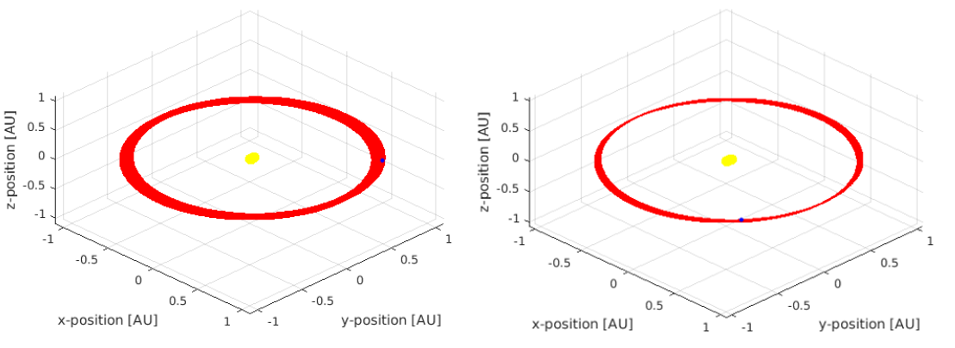
\includegraphics[width=0.99\textwidth]{../figures/earthcompare.png}
	\caption{Figure showing the difference in precision between the Euler-Cromer method (left) and the velocity Verlet method (right). The time step is $dt=10^{-2}$ and the number of points is $N=10^6$\label{fig:earthcompare}}
\end{figure}

The model is easily adjustable and one can modify it to show many interesting phenomena. In figure \ref{fig:earthescape} is a plot showing the Earth escaping its orbit around the sun. The escape velocity was found by trial and error; $v=\sqrt{8}\pi AU/yr$.

\begin{figure}
	\centering
	\textbf{Earth Escape Velocity}
	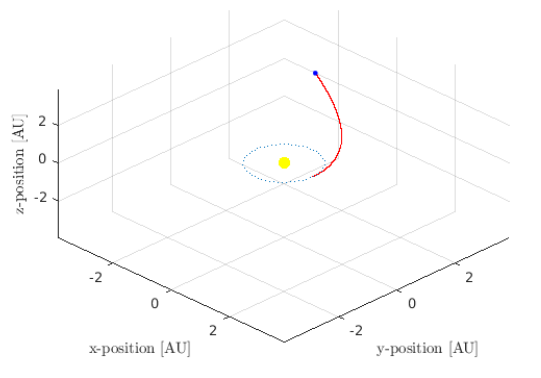
\includegraphics[width=0.9\textwidth]{../figures/earthescape.png}
	\caption{Illustration of Earth escaping orbit at $v=\sqrt{8}\pi AU/yr$\label{fig:earthescape}}
\end{figure}

\begin{table}
	\centering
	\caption{Time comparison of Euler-Cromer and velocity Verlet applied to a two-body system. \label{tab:eulervsverlet}}
	\begin{tabular}{ccc} \hline
	$N$ & Euler-Cromer [t] & Velocity Verlet [t] \\ \hline
	$10^{3}$ & 0.023 & 0.036   \\
	$10^{4}$ & 0.20  & 0.17   \\
	$10^{5}$ & 1.92  & 1.83   \\
	$10^{6}$ & 18.42 & 17.88 \\ \hline
	\end{tabular}
\end{table}

Table \ref{tab:eulervsverlet} shows a comparison of how much time the two algorithm requires to handle a problem of increasing size. The two algorithms were applied to the same two-body problem. As one can see, it appears that the velocity Verlet method is a bit quicker, but these results are probably not statistically significant. More on this in the discussion below.

\subsection{Three-Body system: Earth, Sun and Jupiter}

A natural progression from a two-body system is a three-body system. We have implemented a model consisting of particles representing Jupiter, Earth, and the Sun. The top left subfigure of figure \ref{fig:jupiter} in two dimensions. The velocity Verlet method is employed here.

\begin{figure}
	\centering
	\textbf{Earth, Sun and Jupiter}
	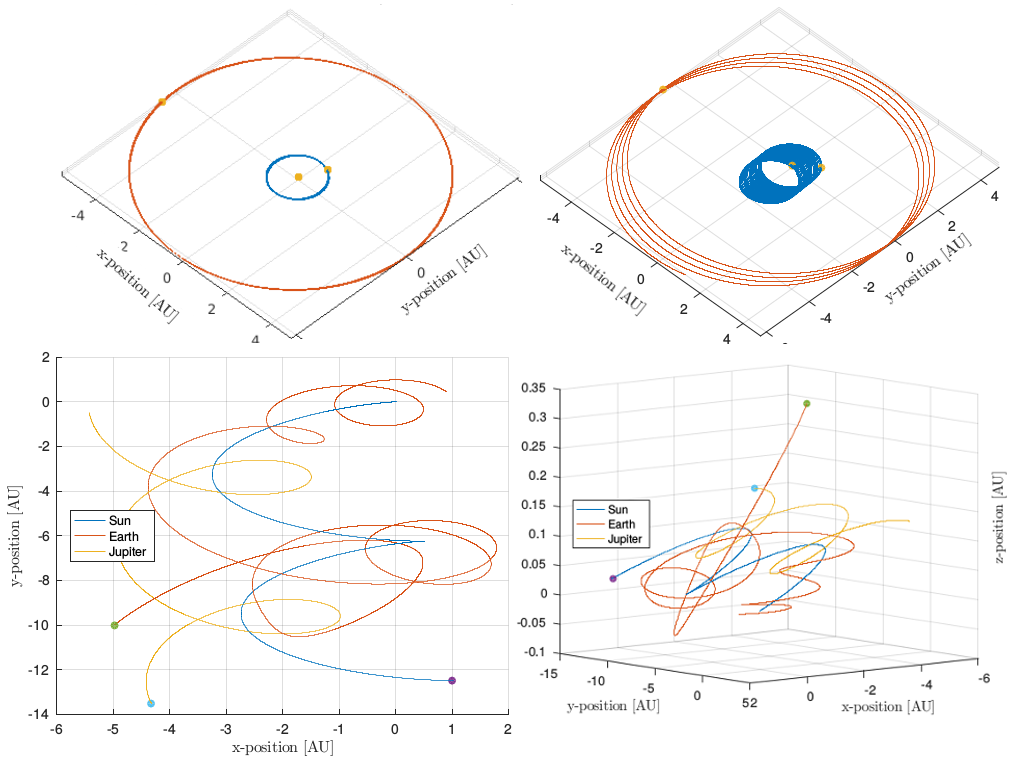
\includegraphics[width=0.99\textwidth]{../figures/threebody.png}
	\caption{Model outcome for a Jupiter with different masses. Top left: Normal mass. Top right: Jupiter mass $10\times$ normal. Bottom: Jupiter mass $1000\times$ normal, in 2D (left) and 3D (right)\label{fig:jupiter}}
\end{figure}

The rest of the subfigures in figure \ref{fig:jupiter} show what would happen if Jupiter had larger mass than it has. The top right subplot shows this scenario if Jupiter's mass was $10\times$ larger than normal. One can see that this would drag the Earth along into the Sun, which stays mostly put, and likely skew the entire solar system.

The two bottom figures show what would happen i Jupiter would have had $1000\times$ normal mass. The plot speaks for itself; the entire system is pulled apart. This situation is shows in 2D to the left and 3D to the right.

\subsection{Multi-Body system: all planets}

\begin{figure}
	\centering
	\textbf{Multi-body model of the Solar System}
	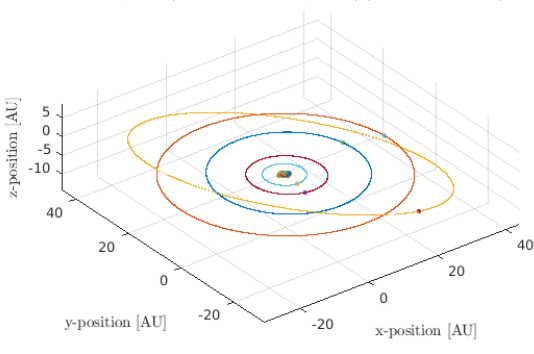
\includegraphics[width=0.9\textwidth]{../figures/multibody.png}
	\caption{All planets of our solar system (including Pluto) \label{fig:multibody}}
\end{figure}

Finally for the pinnacle of this study, a model of the entire solar system!\footnote{Excluding moons and other satelites, but including Pluto.} Figure \ref{fig:multibody} shows a multi-body simulation representing the solar system, integrated using the velocity Verlet algorithm. One can see that the algorithm handles the problem quite well. We were even able to make an anmation of this system in MATLAB, which was a delightful exercise.

\subsection{The perihelion precession of Mercury}

Figure \ref{fig:perangle} shows the angel of the perihelion of Mercury calculated by equation \ref{eq:perangle} in the theory section. This plot is over a period of 30 Earth years and with a time step of $dt = 10^{-6}yrs$. One can see a clear trend in the angle of the perihelion as predicted. We get a slope of the perhelion angle versus number of orbist of approximately $10^{-6}$, for a century on earth Mercury makes $415.2091$ orbits, which gives us a perhelion precession of $\approx1.5''/100yrs$. This much lower than the expected precession of $43''/100yrs$.

\begin{figure}
	\centering
	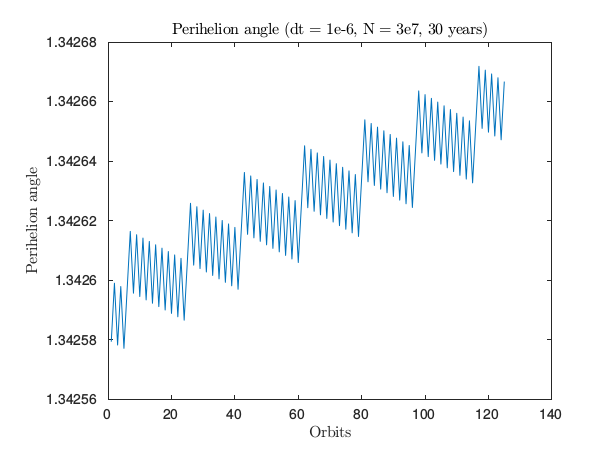
\includegraphics[width=0.8\textwidth]{../figures/periangle30yrs.png}
	\caption{The precession of Mercury's orbit\label{fig:perangle}}
\end{figure}

\section{Discussion}

\subsection{Object Orientation}
This project has been a nice exercise in object oriented thinking. We have built a larger and larger system by adding more class instances and building subclasses such as different integrators. Object oriented programming is close to how we as humans usually thinks about all things in the world. A planet is something that has mass, a position, velocity and some other factors. However, when one learns how to program learns object orientation at a late stage of the learning process, when one has been focusing on a more procedural programming technique.

Most widely used programming languages today are object-oriented to a greater or lesser extent: Java, C++, Python, PHP, Ruby, Smalltalk and Common Lisp, to name a few. Critique of object orientation usually emphasizes that design and modelling comes at the expense of other important aspects like the actual computation and algorithms. The creator of Erlang, Joe Armstrong, is quoted as saying, \say{The problem with object-oriented languages is they've got all this implicit environment that they carry around with them. You wanted a banana but what you got was a gorilla holding the banana and the entire jungle}. 

As fairly level-headed Norwegian patriots\footnote{A friendly reminder to the reader: the creators of the first object oriented languas, Simula, were Norwegian: Ole-Johan Dahl, Kristen Nygaard.} we cannot end the discussion about object orientation there, but rather by pointing out the advantages. Object Oriented Programming provides a clear modular structure for programs and makes it easy to maintain and modify existing code thereby reducing lowering programming ``cost''.

\subsection{Integration Algorithm}

We have seen that the velocity Verlet algorithm is much more precise than the Euler-Cromer method (figure \ref{tab:eulervsverlet}). In addition it appears that it may also be quicker (table \ref{tab:eulervsverlet}), which is a surprise since the Verlet algorithm seems to include more FLOPS than the Euler-Cromer method. This leads us to believe that the velocity Verlet may not be that much faster, at least we can conclude that the results are not statistically significant since we only have one observation per method per value for $N$. An improvement on this study would have been to conduct such a test. We propose larger sampling of code run time and, for simplicity, a paired Student's t-test as a start to answer this question\cite{student}.

The discussion of an Euler method versus a Verlet method is a rather big one. Both methods are quite quick cheap which is what you want, and they are usually the two methods of choice if one does not need entirely exact results, but results that are ``good enough''. A field where this discussion prominent is in physics engine design for video games. With more computing power one would probably go for a more sophisticated method like a foruth degree Runge-Kutta method\cite{physicsengine}.

It is worth metioning something about the symplecticity of the velocity Verlet method. As stated previously, a symplectic method will be good at simulating systems with energy conservation. We believe that the solar system has conserved energy, but our model of it may not be. Looking further into this matter we have found that both energy and angular momentum is conserved for the two-body Earth-Sun system. This would warrant further use of the velocity Verlet scheme. See appendix \ref{app:energy} for a sample readout of energies and angular momenta.

\subsection{Mercury}

We tried to compute the perihelion precessrion of Mercury. We found it to be $\approx1.5''/100yrs$ when it should have been much more, id est $43''/100yrs$. This error can stem from several sources. Most obvious is that we have done something wrong and have been unable to find where. Antoher likely source of uncertainty is that the method is that the integration method is not precise enough. We had problems decreasing the step size further, and extending the simulation to a full century because the job was too much for our hardware. One last probelm that must be mentioned is that Mercury's precession cannot be explained by the simple relativistic correction we are employing.

\section{Conclusion}

\begin{thebibliography}{9}

\bibitem{erlang}
	Armstrong, Joe (2009),
	\emph{Coders at Work: Reflection on the Craft of Programming},
	Peter Seibel, ed.

\bibitem{student}
	Hazewinkel, Michiel, ed. (2001), 
	Student test,
	\emph{Encyclopedia of Mathematics},
	Springer.
	
\bibitem{physicsengine}
	Boesch, Florian (2010, August 28),
	\emph{Integration by Example - Euler vs Verlet vs Runge-Kutta},
	Retrieved October 24 2016 from \url{http://codeflow.org/entries/2010/aug/28/integration-by-example-euler-vs-verlet-vs-runge-kutta/},

\end{thebibliography}

\pagebreak

\begin{appendix}

\section{Class Diagram}
\label{app:classdiagram}

\begin{figure}[ht]
	\centering
	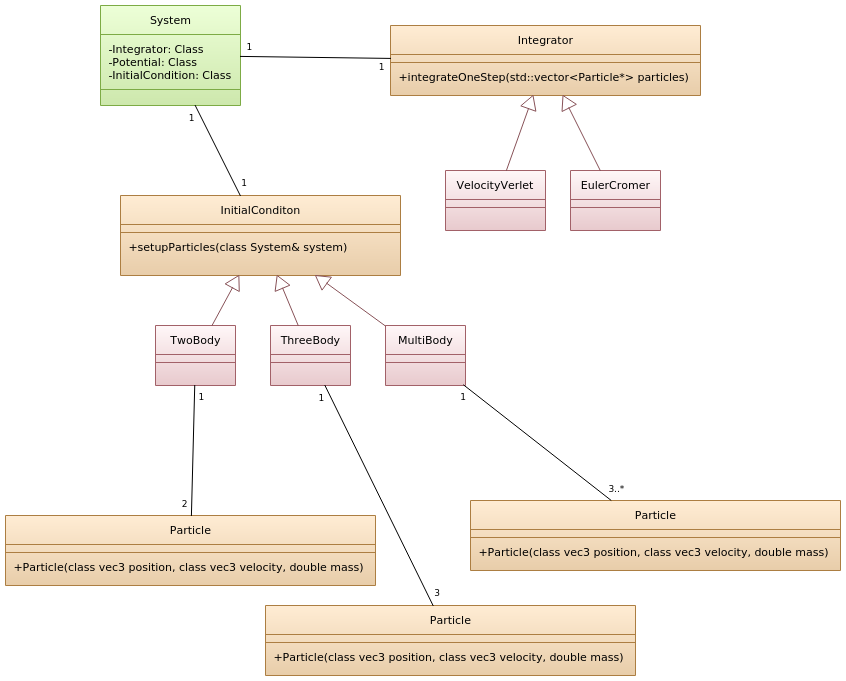
\includegraphics[width=0.9\textwidth]{../figures/classdiagram.png}
\end{figure}

\section{Energy Read-out}
\label{app:energy}
\begin{lstlisting}[keywordstyle=\ttfamily, identifierstyle=\ttfamily]
Energies printed in C++:

Energies for Earth-Sun
EULER-CROMER
Angular momentum: 39.4784*m
Step: 1000000  E = -2e-05   Ek =1.9739e-05  Ep =-3.9478e-05
VERLET
Angular momentum: 39.4784*m
Step: 1000000  E = -2e-05   Ek =1.9739e-05  Ep =-3.9478e-05

Energies for three-body system
Step: 1000000  E = -0.004   Ek = 0.0040197  Ep =-0.0077056
For 10m_j
Step: 1000000  E =  -0.04   Ek =  0.041006  Ep = -0.077361
For 1000m_j
Step: 100000   E =     -4   Ek =     3.314  Ep =    -6.944

Energies for multi-body system dt=1e-5 N=1e5
Step: 100000   E = -0.004   Ek = 0.0040429  Ep =-0.0084804
\end{lstlisting}

\end{appendix}

\end{document}
